Tato kapitola popisuje strukturu souborového systému Zettabyte, jeho základní funkce a rozebírá existující řešení výše popsaného problému.
\section{Souborové systémy}
    Souborový systém je způsob jak organizovat data v datových úložištích. Jak už název napovídá data jsou v úložišti organizována do souborů.
    Tento systém si o každém souboru udržuje informace, aby bylo později možno zjistit, kde se soubor nachází, jak je velký popřípadě jak se jmenuje.

    Způsobů jak data organizovat je mnoho, a proto máme k dispozici mnoho různých souborových systémů. Ty se liší nejenom ve způsobu jak soubory organizují,
    ale také jak velké datové úložiště dokáží adresovat nebo jak velké soubory dokáží spravovat. Další rozlišováním může být závislost na operačním systémů.

    Mezi nejznámější zástupce unixových systémů souborů patří následující systémy
    \begin{itemize}
      \item UFS
      \item ext2, ext3, ext4
    \end{itemize}

    Naopak mezi nejznámější zástupce platformy Windows se řadí navazující systémy
    \begin{itemize}
      \item FAT12, FAT16, FAT32
      \item NTFS
    \end{itemize}

        \subsection{Porovnání}
        Následuje stručné porovnání vybraných souborových systémů z hledska maximální délky názvu souboru, maximální velikosti souboru a maximální velikosti svazku.
        \begin{table}[]
        \centering
        \caption{Porovnání systémů souborů}
        \label{fscompare}
        \begin{tabular}{|l|l|l|l|}
        \hline
        Název & Max. délka názvu & Max. velikost souboru & Max. velikost svazku \\ \hline
        TODO & TODO & TODO & TODO \\ \hline
        \end{tabular}
        \end{table}
\section{Souborový systém Zettabyte}
    %NICM MOC
    Souborový systém Zettabyte byl původně vyvinut společností Sun Microsystems a následně integrován do operačního systémů Solaris od stejnojmenné společnosti.
    Jak už to tak v dnešním světě bývá v roce 2010 společnost Oracle akvizicí společnosti Sun Microsystem získala vlastnicví ZFS i operačního systému Solaris. Veškerý vývoj
    a podpora pro tyto systémy dnes pochází právě od firmy Oracle.

    Systém byl původně navrhnut pro použití čistě v operační systému Solaris s čímž se pojily i minimální požadavky pro provoz ZFS.
    \begin{itemize}
      \item Architektura procesoru SPARC nebo x86
      \item Operační systém Solaris 10 6/06 nebo novější
      \item Minimální místo na disku 128 MB
      \item Minimální místo pro vytvoření poolu 64 MB
      \item Pro optimální výkon ZFS alespoň 1 GB operační paměti
    \end{itemize}
    <CITATE>
    V dnešní době je již bylo ZFS přeneseno i na jiné operačních systém než je Solaris. Jako příklad můžeme vzít operační systém Linux a většinu jeho distribucí <CITATE>

    \subsection{Struktura}
    Většina tradičních souborových systémů se váže na jedno konkrétní zařízení. Aby bylo možné adresovat více zařízení byl zaveden takzvaný volume manager který souborovému
    systému poskytoval iluzi, že se jedná o samostatné zařízení. <CITATE> Ve skutečnosti se pod touto vrstvou mohlo skrývat více disků. ZFS se v tomto směru vydalo opět svojí
    vlastní cestou. Zařízení agreguje do takzvaných poolů, které slouží jako datový základ pro jednotlivé souborové systémy.<IMAGE>
    \subsection{Pool}
    ZFS jako celek se skládá ze dvou hlavních stavebních kamenů. Prvním z nich je takzvaný pool. V terminologii ZFS je to logické sdružení virtuálních zařízeních, které popisuje rozložení a fyzické vlastnosti těchto zařízeních.<CITATE>Pool je tedy jaká si agregace fyzických nebo virtuálních zařízení, která se poskytuje základ pro souborové systémy.

    Souborové systémy v ZFS se už neváží přímo na konkrétní fyzické zařízení jak tomu bylo dříve, ale na pool jako celek. Historické spojení souborového systému s konkrétním fyzickým zařízením přinášela mnohá omezení. Například pokud jsme souborový systém chtěli rozšířit, museli jsme ho celý znovu vytvořit. Tato operace může být časově náročná, ale
    v ZFS tomu tak není.
    \subsection{Vlastnosti poolu}
    ZFS si o každém vytvořeném poolu udržuje infromace, které používá pro správu. Každý pool má tedy seznam vlastnotí, které tento pool popisují a jednoznačně určují.
    Hlavním identifikátorem poolu je jeho jméno. Toto jméno musí být v kontextu celého ZFS unikátní, protože je používáno v příkazech manipulujích s danným poolem.

    Vlastnosti můžeme rozdělit na dvě skupiny. Na jedné straně jsou statické informace, které popisují stav poolu a nedají se změnit přímo. Jsou takzvaně read-only. Pod tímto druhem informací si můžeme představit informace týkající se úložného prostoru jako například velikost, obsazenost a volné místo. Velikost poolu nemůžeme změnit přímo nastavením vlastnosti na jinou hodnotu, ale můžeme přidat do poolu další zdroj, který tuto informaci změní.

    Na druhé straně jsou informace, které můžeme měnit přímo buďto dynamicky, když je pool vytvořen nebo když pool vytváříme nebo importujeme. Nastavit u poolu můžeme například vlastnot readonly, která zajistí, že od doby kdy byla tato vlasnot nastavena lze z daného poolu data pouze číst a nikoliv data zapisovat. Další zajímavou vlastností je vlastnot bootfs, která odkazuje na souborový systém, který slouží pro boot operačního systému. Manuální nastavovaní této vlastnosti se nedoporučuje, protože špatné nastavení může vést k nenačtení operačního systému.

    Pro stručnost jsem z následujícího příkazu, který administrátorovi zobrazuje dostupné infromace o poolu, vybral pouze nejnutnější vlastnoti.
    \begin{verbatim}
    $ zpool get all rpool
    NAME   PROPERTY       VALUE                SOURCE
    rpool  allocated      11.9G                -
    rpool  bootfs         rpool/ROOT/solaris   local
    rpool  capacity       38%                  -
    rpool  dedupratio     1.19x                -
    rpool  delegation     on                   default
    rpool  failmode       wait                 default
    rpool  free           18.9G                -
    rpool  guid           9953515090955426044  -
    rpool  health         ONLINE               -
    rpool  listsnapshots  on                   local
    rpool  readonly       off                  -
    rpool  size           30.8G                -
    rpool  version        37                   default
    \end{verbatim}
    \subsection{Vytváření poolu}
    Výše popsaný pool můžeme v systému kdykoli dynamicky vytvořit bez potřeby jakéhokoli zásahu do systému. Stačí když máme k dizpozici potřebné zdroje (disk, partition, soubor) k vytvoření námi požadovaného poolu. Pokud máme požadované zdroje, stačí už jen vybrat unikátní jméno pro pool v kontextu ZFS a v systému provést například následující příkaz.
    \begin{verbatim}
    $ zpool create tank c1t2d0 c2t1d0
    \end{verbatim}
    V případě dostupnosti disků c1t2d0 a c2t1d0, tento příkaz vytvoří pool jménem tank se zdroji  c1t2d0 a c2t1d0.
    \subsection{Rozšiřování poolu}
    Výhodou architektury poolů je možnost dynamického přidávání fyzických nebo virtuálních zařížení do poolu a tím získáváme možnost dynamického rozšiřování kapacity celého poolu.
    Všechny souborové systémy vytvořené nad jedním poolem, sdílejí jeho prostředky. Tudíž když dojde k rozšíření kapacity poolu, rozšíříme i potenciální kapacitu souborových systémů unvnitř.

    Kapacita poolu se dá rozšířit hned několika typy zařízení. Mezi nejpoužívanější patří disk a partition nebo RAID. ZFS nabízí možnost do poolu přidat soubor jako zdroj.
    Tato možnost se jeví jako velmi výhodná pro testování nebo zkoušení, jelikož jsem ji sám při vytváření této práce mnohokrát využil. V praxy tato možnost znamená přidání další
    vrstvy ( souborového systému ) mezi ZFS a samotný zdroj dat. Tento fakt přináší značné zpomalení, a proto se tato možnost v praxy téměř nevyužívá.

    \subsection{RAID}
    V praxy naopak často používaná možnost jak rozšířit nebo vytvořit pool je pomocí virtuálního zařízení RAID. Tato technologie nám dává možnost rekonstrukce ztracených dat v případě výpadku nějakého disku. Souborový systém nabízí softwarový RAID, který nám umožňuje nad fyzickými zařízeními ( disk, partition, soubor ) vytvářet virtuální zařízení následujících typů.
    \begin{itemize}
      \item RAID1 - zrcadlení
      \item RAIDZ1 - stripování s jendím paritním diskem
      \item RAIDZ2 - stripování se dvěma paritními disky
      \item RAIDZ3 - stripování se třemi paritními disky
    \end{itemize}
    <IMAGE>

    Zrcadlení (RAID1) můžeme pomocí ZFS vytvořit nad dvěma a více zařízeními. Tento typ virtuálního zařízení pak jednoduše replikuje všechny data z disků na všechny ostatní disky
    ve virtuálním zřízení. Pokud zrcadlení vytvoříme nad třemi disky, nakonec budou data na všech třech discích stejná a v případě výpadku jednoho z nich o data nepřijdeme. Jiná situace je samozřejmě v případě výpadku všech třech disků najednou. RAID nám v tomto případě nepomůže a všechny data ztratíme. Nicméně pravděpodobnost, že dojde k výpadku všech
    tří disků najednou, než stihneme alespoň jeden vyměnit, je malá.
    \begin{verbatim}
    $ zpool TODO mirror c1t1d0 c1t2d0 c2t1d0
    \end{verbatim}

    Stripování (RAIDZN) je technika ukládání dat na disk v takzaných stripech. Vezměme v úvahu například virtuální zařízení RAIDZ1 s jedním paritním diskem, do kterého přidáme tři disky. Pokud pokud zapisujeme na toto virtuální zařízení data jsou tyto data rozdělena do stripů. Stripe je základní jednotou zápisu dat a v našem případě se část stripu ukládá na první disk, část na druhý a poslední část na třetí disk. Z dat je vypočtena takzvaná parita, která se následně uloží na paritní disk. Z této hodnoty v případě výpadku jednoho disku dokážeme zpět dopočítat data, která byla uložena na nefunkčním disku. V případě výpadku dvou a více disků najednou o data opět přijdeme. V případě stripování nám RAIDZ přináší i výhodu ve čtení dat z disků. Vzhledem k tomu, že data jsou rozložena na více discích, dokážeme číst z více disků najednou a tím docílit vyšší rychlosti čtení.
    \begin{verbatim}
    $ zpool create raidz1 c1t1d0 c1t2d0 c2t1d0 c2t2d0
    \end{verbatim}

    V případě stripování s více paritními disky jsme schopni obnovit data při výpadku dvou disků při dvou paritních discích atp.. Výhoda vyšší čtecí rychlosti je stále zachována, protože můžeme data načítat z více disků najednou.
    \subsection{Zrušení poolu}
    Stejně jako můžeme dynamicky pool vytvářet a rozšiřovat, můžeme pool i kdykoli zničit a uvolnit tak prostředky, které pool využíval. Tyto prostředky jsou ihned k dispozici a můžeme z nich vytvořit nový pool nebo je použít rozšíření jiného poolu. Jelikož všechny souborové systémy vytvořené nad poolem sdílejí jeho prostředky, jsou tyto souborové systémy zničeny spolu s poolem. Ke zničení poolu, který jsme dříve vytvořili můžeme použít následující příkaz.
    \begin{verbatim}
    $ zpool destroy tank
    \end{verbatim}
    Pokud v systému existuje pool jménem tank, příkaz ho zničí bez ohledu na to kolik souborových systému nad tímto poolem bylo vytvořeno.

    \subsection{Souborový systém}
    Druhým ze stavebních kamenů ZFS jsou samotné souborové systémy. Jak jsem již zmínil dříve, souborový systém je způsob organizace dat do souborů v datových úložištích.
    Tradiční souborové systémy využívají k organizaci různých datových struktur. Souborový UFS využívá takzvaných inodů, což je datová struktura držící attributy souboru a informace o datových blocích. Souborový systém FAT nadruhou stranu využívá takzvané file allocation table. ZFS k tomuto účelu využívá stromové datové struktury, kterou můžete vidět na obrázku <CITATE Struktura>. \begin{figure}[!h]
        \caption{Struktura souborového systému ZFS}
        \label{structure}
    \end{figure}

    Tato stromová struktura přináší zajímavý výhody o kterých si povíme v další kapitolách.
    \subsection{Vlastnosti souborového systému}
    Stejně jako si ZFS udržuje u každého poolu jeho vlastnosti, udržuje si je také u každého souborového systému. Tyto vlastnosti jednoznačně určují souborový systém a popisují jeho chování. Souborový systém je jednoznačně určen svým indetifikátorem, který se skládá z nadřazený souborových systémů včetně poolu a samotného názvu danného systému. Identifikátor by mohl vypadat třeba následovně \emph{rpool/ROOT/solaris}.

    Vlastnosti souborových systému můžeme rozděli stejně jako u vlastností poolu na dvě kategorie. První kategorií jsou vlastnosti, které se dají pouze číst. V této skupině můžeme najít vlasnosti popisující využití místa v souborovém systému. Například kolik místa bylo spotřebováno snapshoty nebo vnořenými souborovými systémy, ale také spotřeba místa souborovým systémem samotným. Ve vlastnostech můžeme také najít poměr deduplikace a komprese nebo datum vytvoření danného souborového systému.

    V duhé kategorii jsou pak vlastnosti, které může administrátor změnit za běhu nebo při vytváření. Stejně jako na úrovní poolu tak i na úrovni souborového systému můžeme nastavit vlastnost readonly, která znemožní uživatelům zapisovat nebo měnit data v souborovém systému. Za zmíňku dále stojí vlastnost exec, která dovoluje v souborovém systému spouštět procesy. O další zajímavých vlastnostech se zmíním v kapitolách Kvóty \ref{quota}, Deduplikace \ref{dedup} a Mountpoint \ref{mount}.

    Administrátor může jednoduše zapínat, vypínat či měnit vlastnosti souborového systému pomocí příkazu \verb|$ zfs set property=value rpool|, popřípadě si zobrazit seznam všech dostupných vlastností o souborovém systému pomocí \verb|$ zfs get all rpool|.

    \subsection{Hierarchie souborových systémů}
    \label{hiararchy}
    Jednou z vlastností ZFS je možnost hieararchického vnořování souborových systémů do sebe. Fakt, že samotný pool jakožto zdroj místa pro souborové systémy se chová jako samostatný souborový systém, tuto vlastnost dokazuje. Přesvědčit se o tom můžeme pomocí následujícího příkazu, kterému místo jéma souborového systému předáme jméno poolu. Pokud příkaz proběhne dobře vypíše základní informace o souborovém systému.
    \begin{verbatim}
    $ zfs list rpool
    NAME    USED  AVAIL  REFER  MOUNTPOINT
    rpool  12.1G  18.2G  4.85M  /rpool
    \end{verbatim}
    Pokud by takovýto souborový systém nexistoval, příkaz by vrátil chybovou hlášku.

    Jelikož pool je vlastně souborový systém a souborové systémy se váží na pool, jde už při vytváření souborového systému vně poolu o hierarchické vnořování. Pool tedy tvoří hlavní uzel v této hierarchické posloupnosti a všechny souborové systémy vytvořené nad tímto poolem jsou jeho potomkem. V jednom poolu můžeme vytvořit více souborových systémů a také je do sebe můžeme libovolně vnořovat. Nejlépe si můžeme tuto hierarchii ukázat na obrázku \ref{fshierarchy}, kde můžeme vidět jak se do sebe jednotlivé souborové systém vnořují.
    \begin{figure}[h]
        \caption{Hierarchie souborových systémů ZFS}
        \label{fshierarchy}
    \end{figure}

    Díky této hierarchické struktuře se dá jednoduše zjistit kdo je předkem danného souborového systému a kdo jeho potomkem. Všechny nastavitelné vlastnosti kromě kvót a rezervací jsou zděděny od rodičovského souborového systému. Pokud žádný rodič nemá vlastnost nastavenou explicitně, je použita standardní hodnota.<CITE Dedicnost>

    Pokud chceme explicitně říct aby některá vlastnost byla zděděna od rodič můžeme použít příkaz \verb|$ zfs inherit property rpool|. Tento příkaz odnastaví dannou vlastnost ze souborového systému a pokusí se převzít hodnotu z rodiče. Pokud v žádném z rodičů není hodnota nastavená explicitně je použita standardní hodnota.
    \subsection{Vytváření souborového systému}
    \label{createfs}
    Vytváření souborových systémů v ZFS je velice jednoduché. Jediné co potřebujeme k vytovření souborového systému je jednoznačný identifikátor. Tento identifikátor se skládá posloupnosti předků oddělená lomítkem od počátečního poolu až po jméno danného souborového systému. Příkaz samotnému vytvoření pak pak může vypadat takto \verb|$ zfs create tank/pool/pool|. Pokud neexistují všichni předchůdci je potřeba použít přepínač \verb|-p| jinak příkaz selže.

    Při vytváření je možné specifikovat, které vlastnosti danný souborový systém bude mít. Mimo jiné existuje vlasnost encryption, která se dá nastavit pouze při vytváření. Po vytvoření souborového systému je vlastnost vedena jako readonly a nedá se změnit. Vlastnost encryprion umožnuje šifrování souborového systému pomocí různých kryptografických funkcí jako je například AES. Vlastnost encryption můžeme při vytváření dospecifikovat následovně.
    \begin{verbatim}
    $ zfs create -o enryption=on tank/pool/pool
    \end{verbatim}
    \subsection{Zrušení souborového systému}
    Rušení souborových systému je v ZFS stejně snadné jako jejich vytváření. Je důležité mít na paměti, že zrušením souborového systému, který má nějaké potomky, zrušíme i všechny jeho potomky. Pro samotné zrušení souborového systému pak již stačí vyvolat příkaz \verb|$ zfs destroy| s příslušným identifikátorem popřípadě přepínačem \verb|-r| pro zrušení všech potomků.
    \subsection{Kvóty}
    \label{quota}
    %% Kvóty
    Kvóty v ZFS umožňují administrátorovi spravovat limity souborových systémů týkajících se využitého místa. Tyto limity tedy omezují možnosti využití dostupného místa v souborovém systému. Kvóty můžeme rozdělit do následujících kategorií podle toho koho omezují.
    \begin{itemize}
      \item Obecné - týkající se souborového systému
      \item Uživatelské
      \item Skupinové
    \end{itemize}

    Obecné kvóty tedy omezují místo, které může využít souborový systém jako celek. K tomuto účelu v ZFS slouží vlastnost \emph{quota} u každého souborového systému, která stanovuje limit místa, které může danný souborový systém využít. V tomto případě se do využitého místa započítává i místo spotřebované potomky. <CITE Quota> Pokud bychom chtěli omezit souborový systém bez ohledu na to kolik místa využijí jeho potomci musíme použít vlastnost \emph{refquota}.
    %% Rezervace

    Vzhledem k faktu, že souborové systémy v jednom poolu sdílí dískové místo, ZFS přichází s vlastností \emph{reservation}. Tato vlastnost oproti kvótám garantuje souborovému systému diskové místo danné velikosti. <CITE Quota> Stejně jako v případě vlastnosti \emph{quota} je toto místo vyhrazeno pro souborový systém a věechny jeho potomky. Pokud bychom chtěli garantovat místo přímo souborovému systému, bez ohledu na to kolik místa využívají jeho potomci, musíme využít vlastnost \emph{refreservation}.

    Jelikož vlastnosti \emph{quota} resp. \emph{refquota} a vlastnosti \emph{reservation} resp. \emph{refreservation} jsou vlastnostmi souborového systému, můžeme je nastavit stejně jako jakoukoli jinou vlastnost pomocí následujících příkazů.
    \begin{verbatim}
    $ zfs set quota=10G rpool/export/home
    $ zfs set reservation=10G rpool/export/home
    \end{verbatim}

    Vztahy mezi vlastnostmi \emph{quota} a \emph{reservation} jsou vyznačeny na obrázku \ref{quotavsreserv}.
    %% Obrázek
    \begin{figure}[h]
        \caption{Vztahy mezi vlastnostmi \emph{quota} a \emph{reservation}}
        \label{quotavsreserv}
    \end{figure}
    %% Uživatelské a skupinové kvóty

    Další možností jak omezit využití diskového místa je pomocí uživatelských resp. skupinových kvót. Tyto kvóty limitují uživatele resp. skupinu v tom, kolik místa můžou na souborovém systému využít. Každý souborový systém má svůj vlastní \emph{userspace} resp \emph{groupspace}, kde si udržuje informace o tom jaké limity jednotlivý uživatelé resp. skupiny mají.
    Administrátor si může hodnoty uživatelský resp. skupinových kvót vypsat pomocí \verb|$ zfs userspace filesystem| resp. \verb|$ zfs groupspace filesystem|. Následující příkaz demonstruje jak vypadá výpis uživatelských kvót pro domací adresář.
    \begin{verbatim}
    $ zfs userspace rpool/export/home/simactom
    TYPE        NAME       USED  QUOTA  SOURCE
    POSIX User  root      1.50K   none  default
    POSIX User  simactom   641M   none  default
    \end{verbatim}

    Pokud se uživatel resp. skupina v seznamu nenachází nebo je u něj uvedena hodnota \emph{none}, uživatelské resp. skupinové kvóty se na něj nevztahují. Je-li v seznamu uvedena hodnota, pak uživatel v danném souborovém systému nesmí překročit tuto hodnotu. Pokud by tuto hodnotu překročil systém ho varuje a požadovanou akci neprovede. Přiřazení kvóty uživately resp. skupině provedeme pomocí následujících příkazů
    \begin{verbatim}
    $ zfs userquota@username=value filesystem
    $ zfs groupquota@username=value filesystem
    \end{verbatim}

    ZFS nabízí ještě vlastnost \emph{defaultuserquota} resp. \emph{defaultgroupquota}, kterou lze nastavit na určitou hodnotu. Tento limit se použije v případě, že hodnotu uživatelské resp. skupinové kvóty nastavíme na \emph{default}.
    \subsection{Deduplikace}
    \label{dedup}
    Jednou z další vlastností, které ZFS nabízí je deduplikace. Jak již z názvu vyplívá, jedná se o proces, který zabraňuje duplikaci dat na disku a tím šetří místo na disku. Deduplikace se obecně dá rozdělit na následující úrovně.
    \begin{itemize}
      \item Úroveň souborů
      \item Úroveň datavých bloků
      \item Úroveň bytů
    \end{itemize}

    K identifikaci stejných souborů, datových bloků nebo bytů se využívá hašovácí funkce. Data jsou pomocí této funkce zahešována a výsledné haše porovnány na rovnost. Pokud se haše rovnají a používáme hašovací funkci SHA256, můžeme s pravděpodobností , že se data opravdu rovnají.<CITATE Deduplikace> Pokud je administrátor z nějakého důvodu stále nedůvěřivý může u vlastnosti deduplikace nastavit hodnotu \emph{verify}, která zajistí celkové porovnání datových částí se 100\% pravděpodobností.

    Deduplikace na úrovni souborů využívá nejméně systémových prostředků, protože se data hašují a porovnávají po velký částech. Na druhou stranu sebemenší změna v souboru vyžaduje přepočítání haše, který se již bude lišit od původního.<CITATE Deduplikace> Souborový systém pak rozpozná že se soubory liší a uspořené místo bude zaplněno změněným souborem.

    Deduplikace datových bloků vyžaduje oproti deduplikaci souborů vyšší využití systémových prostředků, ale na druhou stranu přináší v jistých situacích lepší úsporu místa. <CITATE Deduplikace>
    V poslední řadě existuje deduplikace na urovni bytů je ze všech uvedených úrovní nejnáročnější na využití prostředků. Tato možnost se používá jen ve speciálních případech.

    ZFS z výše uvedených možností nabízí právě deduplpikaci na úrovni datových bloků, protože tato jednotka deduplikace přináší nejvíce výhod v obecných případech použití.<CITATE Deduplikace> Na obrázku \ref{blockdedup} můžeme vidět, jak dochází k úspoře místa pokud je v ZFS souborovém systému zapnutá vlastnost \emph{dedup}.
    \begin{figure}[!h]
        \caption{Ukázka deduplikce na úrovni datový bloků}
        \label{blockdedup}
        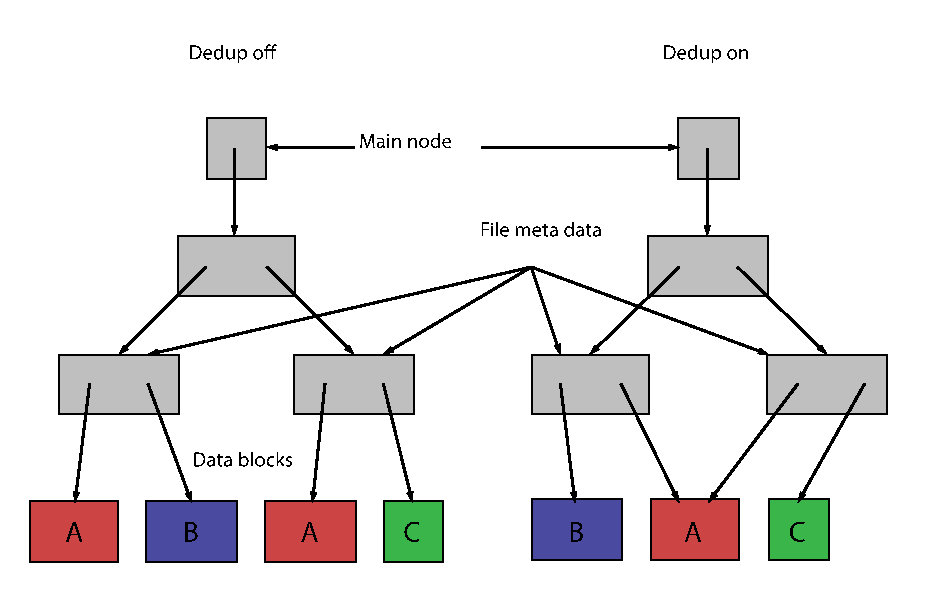
\includegraphics[scale=0.8]{dedup.pdf}
    \end{figure}
    \subsection{Konzistence}
    \label{consitence}
    Starší souborové systémy jako například UFS zapisují data přímo do bloku, který mění. To může v některých případech, jako je selhání systému nebo výpadek proudu, vést k nekonzistenci souborového systémů. V takovém případě je nutné celý souborový systém zkontrolovat napříkald pomocí příkazu <code>fsck. Bohužel ani ten v některých případech
    nedokáže některé nekonzistence opravit. <CITATE>

    Některé systémy souborů využívají žurnálů k udržení konzistence. Žurnál jse speciální záznam kam se ukládá co a kde se bude měnit, poté
    je provedena vlastní akce. A v poslední fázi se do žurnálu zapíše, že akce byla provedena. Když systém zkolabuje v jakémkoli kroku, je možné ho při startu například pomocí
    fsck dostat opět do konzistentního stavu.

    ZFS přichází s transakčním systémem a technikou copy on write. Tato technika zajišťuje neustálou konzistenci souborového systému i v okamžiku výpadku, a proto není třeba žurnálu. Data na disku nejsou nikdy přímo přepisována.

    Transakce může vypadat následovně. Nejprve dojde ke zkopírování bloků, které mají být změněny. Poté dojde kopii a změně metadat, které se týkají změněných bloků. V poslední
    řadě dojde k atomické operaci, která připojí větev s novými resp. změněnými bloky do stromu souborového systémů. Přůběh transakce je naznačet na obrázku \ref{cow}. Pokud v průběhu transakce dojde k výpadku celý souborový systém zůstává konzistentní, protože nebyla provedena atomická operace připojení k hlavnímu stromu.
    \begin{figure}[h]
        \caption{Demostrace copy on write}
        \label{cow}
        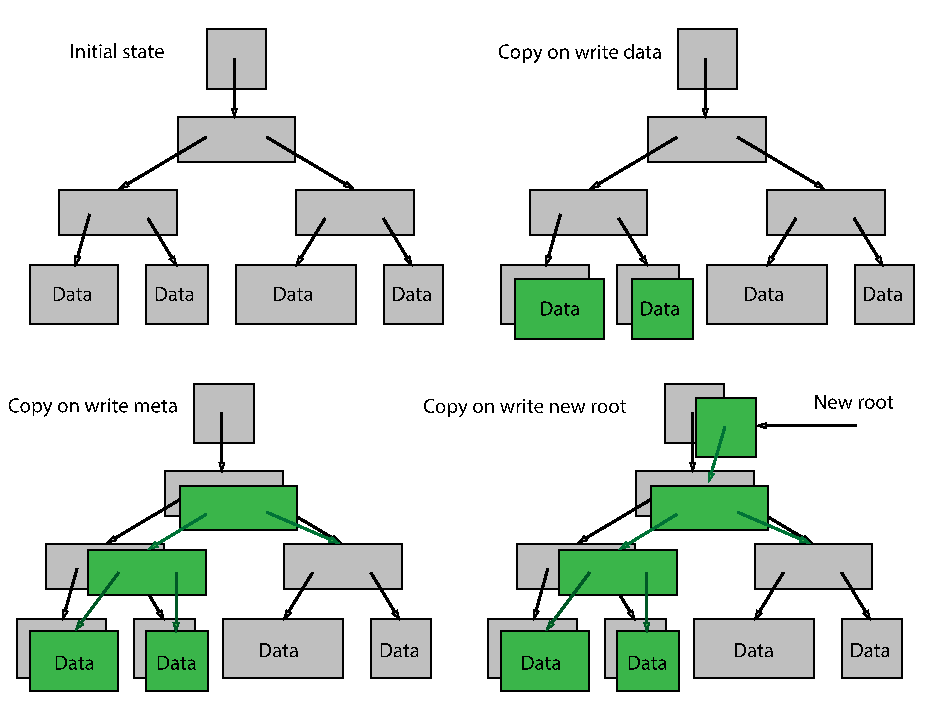
\includegraphics[scale=0.8]{cow.pdf}
    \end{figure}
    \subsection{Integrita dat}
    \label{checksum}
    Od souborového systému očekáváme, že při čtení dat z určitého datového bloku z disku, dostame data, která do tohoto bloku byla dříve zapsána. Pokud tomu tak není, měl by to souborový systém detekovat a vrátit chybu.<CITATE Integrity>

    Vlastnost neustálé konzistence souborového systému ZFS, zmíněná výše v kapitole \ref{consitence}, zajišťuje, že chybná data se v souborovém systému mohou vyskytnout jen skrze hardwarovou chybu. <CITATE integrity2>

    ZFS dokáže tyto chyby hardwaru detekovat pomocí tzv. kontrolních součtů. Tyto součty vznikají a jsou přepočítávány při každé změně bloku v souborovém sytému. Jak jsme mohli vidět na obrázku \ref{structure}, součty nejsou uloženy v bloku, kterého se týkají, ale v bloku jemu nadřazeném. Při každém požadavku na čtení dojde k vypočítání kontrolního součtu na základě dat, které se v souborovém systému momentálně nachází a poté dojde k porovnání vypočteného součtu se součtem uloženým v nadřzeném bloku.<CITATE integrity> Tím ZFS dokáže rozhodnout zda je blok požkozený či nikoliv.

    Díky těmto kontrolním součtům se souborový systém dokáže v určitých situacích sám opravovat. Tato situace nastává v případě, že blok, při jehož čtení došlo k chybě, je součástí redundatního virtuálního zařízení jako je například RAID-Z nebo mirror. V tomto případě ZFS přečte datový blok i z replikovaného disku popřípadě sestaví blok pomocí parity a následně opraví chybný blok, při jehož čtení došlo k chybě. Aplikace dostane správná data i přes to, že při prvním čtení došlo k chybě. Obrázek \ref{selfhealing} názorně ukazuje postup při detekci chyby.
    \begin{figure}[h]
        \caption{Demostrace samopravování}
        \label{selfhealing}
    \end{figure}

    Ačkoliv dochází k ověřování integrity dat automaticky při každém čtení z disku, je možné tento proces manuálně vyvola o věřit pomocí následující sekvence příkazů.
    \begin{verbatim}
    $ zpool scrub pool
    $ zpool status pool
    pool: pool
    state: ONLINE
    scan: scrub repaired 0 in 6s with 0 errors on Thu Apr 21 07:19:59 2016
    \end{verbatim}

    \subsection{Mountpoint}
    \label{mountpoint}
    Mounpoint je jednou ze základních vlastností všech souborových systémů. Je to vlastně cesta k bodu v adresářovém stromu operačního systému, kde má danný souborový systém být připojen.

    Jelikož se ZFS snaží administrátorům maximálně ulehčit práci, stará se o automatické připojování souborových systémů samo. K účelům připojování souborových systémů v ZFS slouží jejich vlastnost \emph{mountpoint}, kde administrátor může specifikovat, kam se má danný souborový systém připojit. Pokud administrátror tuto vlastnost explicitně neurčí, je odvozena od vlasnosti rodičovského souborového systému.

    Pro připojování souborových systémů ZFS se dají použít i tradiční nástroje \emph{mount} a \emph{umount}. V tradičních souborových systémech jako je například UFS se pro automatické připojování používal soubor \emph{/etc/vsfstab}, kdeadministrátor specifikoval co a kam se má připojit. Operační systém po startu tento soubor zpracoval da vyznačené souborové systémy připojil.

    Jak jsem již zmínil ZFS proces automatického připojování provádi samo. Pokud by administrátor chtěl využívat automatického připojování pomocí souboru \emph{/etc/vsfstab}, je možné nastavit vlastnost \emph{mountpoint} souborového systému na hodnotu \emph{legacy}.<CITATE Mountpoint> Tím administrátor řekne, že se o souborový systému bude starat sám a ZFS ho již automaticky připojovat nebude.
    \subsection{Snapshot}
    \label{snapshot}
    ZFS snapshot je stav danného souborového systému v čase, kdy byl snapshot pořízen. Jedná se tedy o kopii danného souborového systému, která se nedá měnit. Je takzvaně readonly.<CITATE Snapshot>
    
    Díky stromové architektuře souborového systému ZFS je pořizování těchto kopií velice elegantní a nenáročné. Pro vytvoření snapshotu můžeme použít příkaz \verb|$ zfs snapshot filesystem@snapshot|, kde \emph{filesystem} je jméno souborového systémů, jehož stav chceme zachytit a \emph{snapshot} je jméno konkrétního stavu.
     
    Po provední příkazu k vytvoření snapshotu dojde ke zkopírování kořene souborového systému jehož snapshot tovříme. Tento kořen se stane havním kořenem snapshotu jakožto nového souborového systému. V tuto chvíli máme k dispozici dva odkazy na jeden souborový systém. Jelikož snapshot je souborový systém určený pouze ke čtení, nemůžeme pomocí něj zmenit data v aktivním souborovém systému. Velikost snapshotu je v tuto chvíli nulová, protože nedošlo k žádnému kopírování dat. Pokud se ovšem data v aktivním souborovém systému změní, je nutné aby snapshot stále odkazoval na stará data. Toho docílíme tak, že stará data zkopírujeme a zvětšíme tak velikost snapshotu.<CITATE Snapshot> Rozšiřování velikosti snapshotu tedy závisí na množství změněných dat od chvíle, kdy byl snapshot vytvořen. Proces vytváření snapshotu a rozšiřování jeho velikosti je názorně ukázán na obrázku \ref{snapshotproces}.
    \begin{figure}[h]
        \caption{Vytváření snapshotu}
        \label{snapshotproces}
    \end{figure}
    
    Rekurivní tvorba snapshotů se provádí rychle pomocí jedné atomické operace. Snapshoty jsou vytvořeny naráz všechny dohromady nebo vytvořeny vůbec. Výhodou atomické operace je fakt, že data ve všech snapshotech jsou konzistentní vzhledem k jednomu časovému okamžiku.<CITATE Snapshot>
    
    Snapshot pro souborový systém a všechny jeho potomky můžeme vytvořit pomocí následujícího příkazu.
    \begin{verbatim}
    $ zfs snapshot -r rpool/export/home@snap
    $ zfs list -t snapshot -r rpool/export/home
    NAME                             USED  AVAIL  REFER  MOUNTPOINT
    rpool/export/home@snap              0      -    33K  -
    rpool/export/home/simactom@snap     0      -   641M  -
    \end{verbatim}
    Druhý příkaz v pořadí pak ukazuje skutečnost, že se snapshoty opravdu vytvořili i pro všechny potomky danného souborového systému a že je jejich velikost opravdu nulová.
    
    Snapshot se dá použít k navrácení souborového systému do stavu, v jakém se nacházel v okmažiku vytvoření snapshotu. Veškeré změny, které proběhly v souborovém systému od vytvoření snapshotu budou smazány. K vyvolání tohoto procesu stačí použít příkaz \verb|$ zfs rollback snapshot |, kde \emph{snapshot} je celé jméno snapshotu. Jelikož se každý snapshot váže přímo s určitým souborovým systémem, není třeba zadávat jméno souborového systému, který chceme navrátit do původního stavu.
    
\section{Rozbor existujících řešení}
    V následující kapitole jsem si vybral několik nástrojů sloužící pro monitorování a správu souborového systému ZFS, které se pokusím popsat.
    \subsection{zfsmon}
    Jedním z nástrojů, které jsem si vybral, je \emph{Zfsmon}. Tento nástroj slouží pro monitorování ZFS souborových systémů na více oddělených souborových serverch. Aplikace má dvě oddělené části.
    
    První částí je script, který běží na počítači se souborovým systémem ZFS, který chceme monitorovat. Tento script je spouštěn pomocí crontabu a zajišťuje aktualizaci informací v databázi, která je součástí webové aplikace. Crontab je program, který zajišťuje automatické spouštění scriptů v systému. Doporučený interval spouštění scriptu je 15 minut.<CITATE Zfsmon>
    
    Druhou částí aplikace zfsmon je samotná webová aplikace, která se stará o zobrazování dat z databáze. V databázi se nacházejí informace o stavu jednotlivých souborových systémů z různých serverů. Aplikace zobrazuje informace klientovi na požádání v podobě HTML stránek.
    
    Velkou výhodou této aplikace je, že dokáže zobrazovat informace z více oddělených úložišť najednou. Nadruhou stranu způsob zpracování dat přináší značnou nevýhodu, která spočívá v intervalu aktualizace dat v databázi. V průběhu tohoto intervalu aplikace znemožňuje uživateli vidět aktuální data ze ZFS úložiště. Uživatel je nucen počkat na konec tohoto intervalu, kdy jsou opět nahrána aktuální data do databáze. Další nevýhodou toho nástroje je absence veškeré funkcionality, která by s týkala administrace souborového systému ZFS.
    
    Tento nástroj nám tedy umožňuje kvalitně monitorovat informace z více zdrojů najednou, ale neposkytuje nám možnost jakékoli administrace minitorovaných souborových systémů.     
    \subsection{zfswatcher}
    Jen ve stručnosti zmíním pár informací o nástroji jménem \emph{Zfswatcher}.
     
    Tento nástroj slouží jako webové rozhraní pro sledování souborových systémů ZFS. Stejně jako předchozí nástroj zpracovává periodicky data a zobrazuje je pomocí HTML stránek, s čímž souvisí stejný problém, který jsem popsal u předchozího nástroje. Oproti nástroji \emph{Zfsmon} umí zobrazovat informace pouze z jednoho souborového serveru. Nadruhou stranu tento nástroj umí v případě změny nějaké informace poslat upozornění v podobě e-mailu nebo zalogování do logu.<CITATE zfswatcher>
    \subsection{ZFS administration console}
    Na závěr této kapitoli bych chtěl jen zmínit nástroj \emph{smcwebserver}. Tento nástroj je součástí operačního systému Solaris 10 6/06 a umožňuje administrátorovi spravovat některé funkce tohoto operačního systému. Mimo jiné se část tohoto nástroje věnuje právě správě souborového systému ZFS. Bohužel v novější verzi Solarisu 11 se tento nástroj již nevyskytuje.         